\esSezione{Shift register}\label{sec:esercizio4-1}

\begin{traccia}
Progettare, implementare in VHDL e testare mediante simulazione un registro a scorrimento di N bit in grado di shiftare a destra o a sinistra di un numero Y variabile di posizioni a seconda di una opportuna selezione. In particolare, i valori possibili di Y sono 1 e 2. L'utente tramite selezione deve scegliere di quante posizioni shiftare. Il componente deve essere realizzato utilizzando sia un a) approccio comportamentale sia un b) approccio strutturale. Nota: il numero di bit del registro deve essere implementato come un generic, e dall'esterno deve poter essere scelta la modalità di funzionamento mediante opportuni segnali di selezione.
\end{traccia}

\progetto

Il registro è descritto da un'unica entità, \texttt{shift\_register}, dotata di due architetture: \texttt{Behavioral} e \texttt{structural}. Le due condividono la stessa interfaccia, per poterle istanziare entrambe nel testbench e confrontarne le uscite. Il generic \texttt{N} fissa la larghezza; gli ingressi \texttt{dir} e \texttt{pos} selezionano rispettivamente il verso (\texttt{'0'} destra, \texttt{'1'} sinistra) e il numero di posizioni (\texttt{'0'} una, \texttt{'1'} due), mentre \texttt{en} abilita lo scorrimento e \texttt{load} il caricamento parallelo del dato \texttt{d}. Il reset \texttt{rst} è sincrono e ha la precedenza su \texttt{load}, che a sua volta ha la precedenza su \texttt{en}. Nello scorrimento i bit che entrano valgono \texttt{'0'}.

\subsection*{}
\esSottosezione{Approccio comportamentale}

\implementazione

L'architettura \texttt{Behavioral} contiene un solo process con sensitivity list limitata a \texttt{clk}, attivo sul fronte di salita. Il registro interno \texttt{r} viene azzerato se \texttt{rst} vale \texttt{'1'}, altrimenti caricato con \texttt{d} se \texttt{load} vale \texttt{'1'}; se invece è attivo \texttt{en}, viene aggiornato con una concatenazione che dipende da \texttt{dir} e \texttt{pos}, ad esempio \texttt{'0' \& r(N-1 downto 1)} per lo scorrimento a destra di una posizione. Se nessun controllo è attivo il valore si mantiene. Un'istruzione \texttt{assert} controlla in fase di elaborazione che \texttt{N} sia almeno 2; l'uscita \texttt{q} è assegnata in modo concorrente a \texttt{r}. Si riportano di seguito l'entità e la prima architettura.

\vhdlfile[firstline=1,lastline=52]{esercizio4-1/shift_register.vhd}{Implementazione comportamentale dello shift register}{lst:esercizio4-1:shift-register-beh}

\esSottosezione{Approccio strutturale}

\progetto

La versione strutturale replica per ogni bit una slice, illustrata nella figura~\ref{fig:esercizio4-1:rtl}. Il flip-flop D è preceduto da due multiplexer 2:1 in cascata e da un multiplexer 4:1. Il multiplexer 4:1 sceglie il nuovo valore del bit tra i quattro bit adiacenti (a distanza 1 e 2, a destra e a sinistra) in base a \texttt{dir} e \texttt{pos}; il primo multiplexer 2:1 sceglie tra questo valore e il dato \texttt{d(i)} in base a \texttt{load}; il secondo mantiene il valore corrente \texttt{r(i)} quando né \texttt{load} né \texttt{en} sono attivi, ed è comandato dal segnale \texttt{we}, ottenuto come \texttt{load or en}. 
\begin{figure}[H]
  \centering
  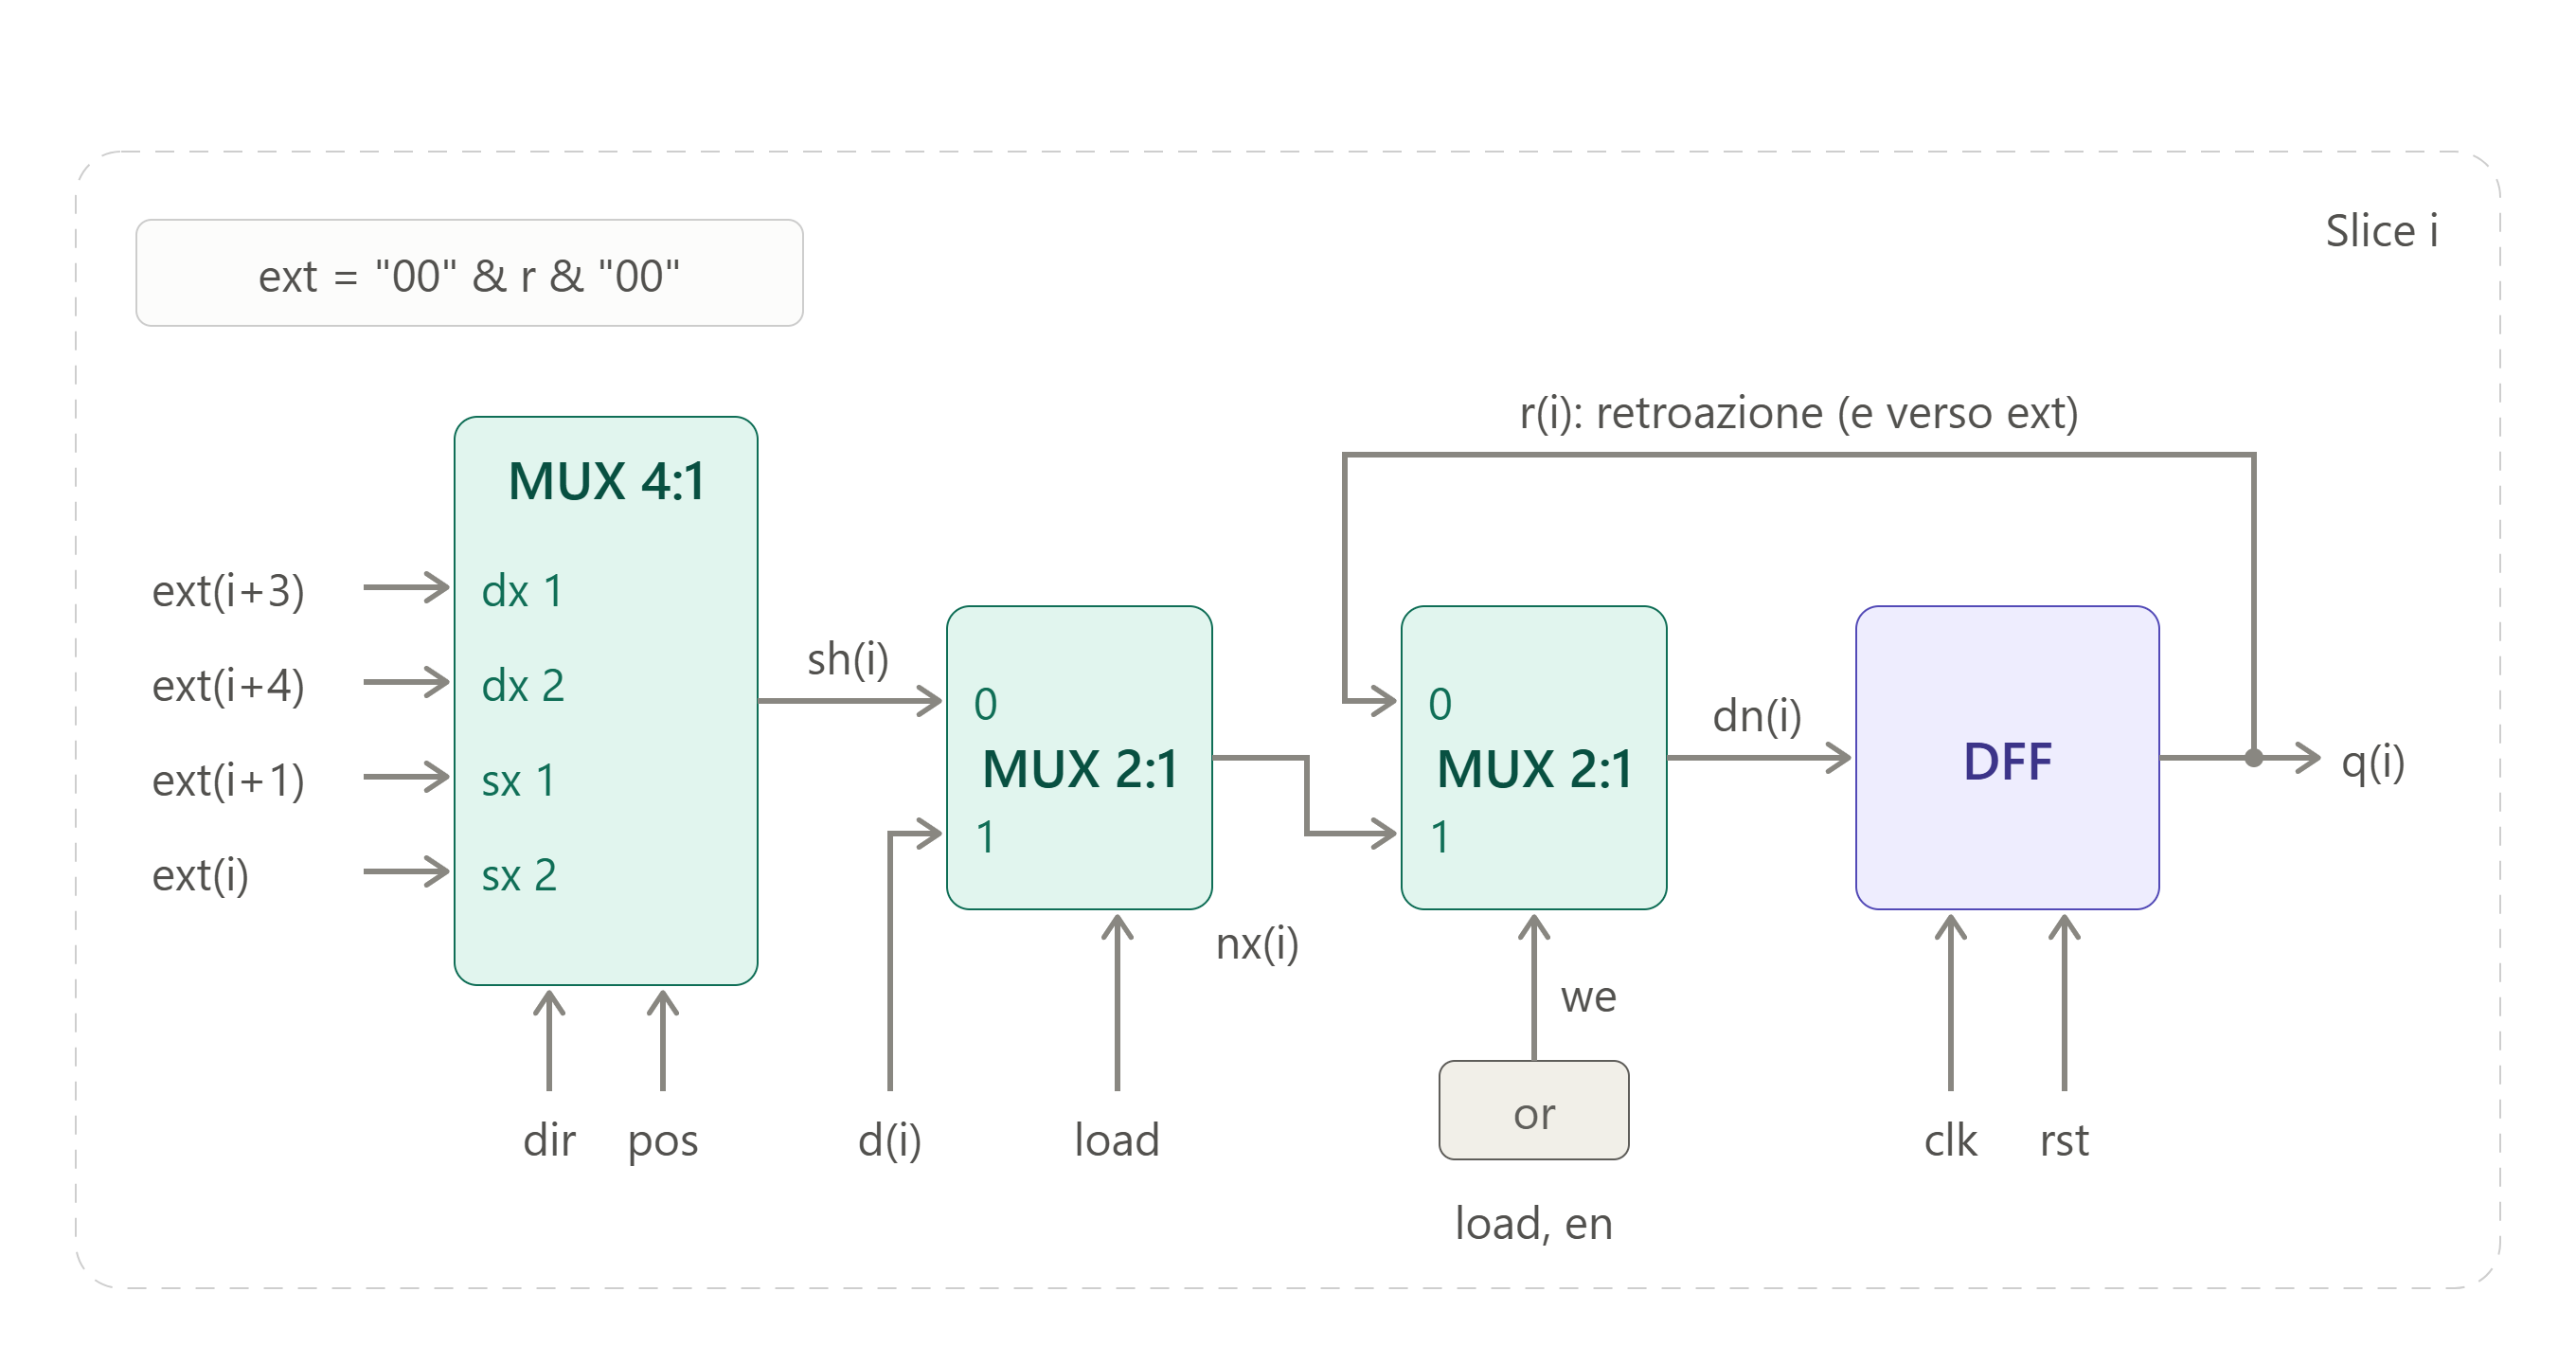
\includegraphics[width=0.75\linewidth]{figure/esercizio4-1/rtl}
  \caption{Slice i-esima dello shift register strutturale}
  \label{fig:esercizio4-1:rtl}
\end{figure}

Per gestire i bit di bordo, il segnale \texttt{ext}, di $N+4$ bit, è ottenuto affiancando due zeri a ciascun estremo di \texttt{r}; in questo modo \texttt{ext(i+3)} e \texttt{ext(i+4)} corrispondono a \texttt{r(i+1)} e \texttt{r(i+2)}, mentre \texttt{ext(i+1)} ed \texttt{ext(i)} corrispondono a \texttt{r(i-1)} e \texttt{r(i-2)}, e i bit fuori dal registro valgono \texttt{'0'}.

\implementazione

Il flip-flop D è l'entità \texttt{dff}, con ingressi \texttt{clk}, \texttt{rst} e \texttt{d} e uscita \texttt{q}, tutti a un bit. L'architettura \texttt{behavioral} è un process sul fronte di salita del clock, con reset sincrono che porta l'uscita a \texttt{'0'}.

\vhdlfile{esercizio4-1/dff.vhd}{Implementazione flip-flop D}{lst:esercizio4-1:dff}

Il multiplexer 2:1 è l'entità \texttt{mux\_2\_1}, con ingressi \texttt{a0} e \texttt{a1}, selezione \texttt{s} e uscita \texttt{y} (usiamo la semplice architettura \texttt{dataflow}).

\vhdlfile{esercizio4-1/mux_2_1.vhd}{Implementazione MUX 2:1}{lst:esercizio4-1:mux-2-1}

Il multiplexer 4:1 è già stato presentato nel listato~\ref{lst:esercizio1-1:mux-4-1} dell'esercizio~1.1; qui si usa l'architettura \texttt{dataflow}.

L'architettura \texttt{structural} dichiara i segnali \texttt{r} (uscite dei flip-flop), \texttt{ext}, \texttt{sh} (uscite dei multiplexer 4:1), \texttt{nx} (valore scelto tra scorrimento e caricamento), \texttt{dn} (ingresso dei flip-flop) e \texttt{we}. Un ciclo \texttt{for generate} istanzia, per ciascun indice \texttt{i}, i componenti \texttt{m\_shift}, \texttt{m\_load}, \texttt{m\_hold} e \texttt{ff} con port mapping. Nel multiplexer 4:1 la selezione è composta da \texttt{dir} (bit più significativo) e \texttt{pos} (bit meno significativo), per cui i valori \texttt{"00"}, \texttt{"01"}, \texttt{"10"} e \texttt{"11"} corrispondono a scorrimento a destra di 1, a destra di 2, a sinistra di 1 e a sinistra di 2. Il reset è collegato ai flip-flop, mentre l'uscita \texttt{q} è assegnata a \texttt{r}. Il codice è il seguente.

\vhdlfile[firstline=54,lastline=95]{esercizio4-1/shift_register.vhd}{Implementazione strutturale dello shift register}{lst:esercizio4-1:shift-register-str}

\simulazione

Il testbench \texttt{shift\_register\_tb} ha entità senza porte e fissa \texttt{N} a 8 e il periodo del clock a \SI{10}{ns}. Sono istanziate due copie del componente, \texttt{dut\_beh} con architettura \texttt{Behavioral} e \texttt{dut\_str} con architettura \texttt{structural}, collegate agli stessi ingressi e con uscite distinte \texttt{q\_beh} e \texttt{q\_str}. Il process \texttt{clk\_proc} genera il clock; il process \texttt{stim} applica gli stimoli; il process \texttt{check} confronta le due uscite a ogni fronte di discesa e segnala con \texttt{assert} l'eventuale divergenza. I passi di prova sono i seguenti.

\begin{enumerate}
  \item Reset per due periodi, con \texttt{rst} a \texttt{'1'}.
  \item Caricamento parallelo di \texttt{"10110011"} (0xB3).
  \item Con \texttt{en} a \texttt{'1'}, quattro scorrimenti consecutivi: destra di 1, destra di 2, sinistra di 1, sinistra di 2.
  \item Mantenimento del valore con \texttt{en} a \texttt{'0'} per due periodi.
  \item Attivazione simultanea di \texttt{load} ed \texttt{en} con \texttt{d} pari a \texttt{"11110000"} (0xF0): prevale il caricamento.
  \item Attivazione simultanea di \texttt{rst} e \texttt{load}: prevale il reset.
\end{enumerate}

\vhdlfile{esercizio4-1/shift_register_tb.vhd}{Testbench dello shift register}{lst:esercizio4-1:tb}

Il risultato della simulazione è mostrato in figura~\ref{fig:esercizio4-1:simulazione}, dove sono visibili anche i singoli bit di \texttt{q\_str}.

\begin{figure}[H]
  \centering
  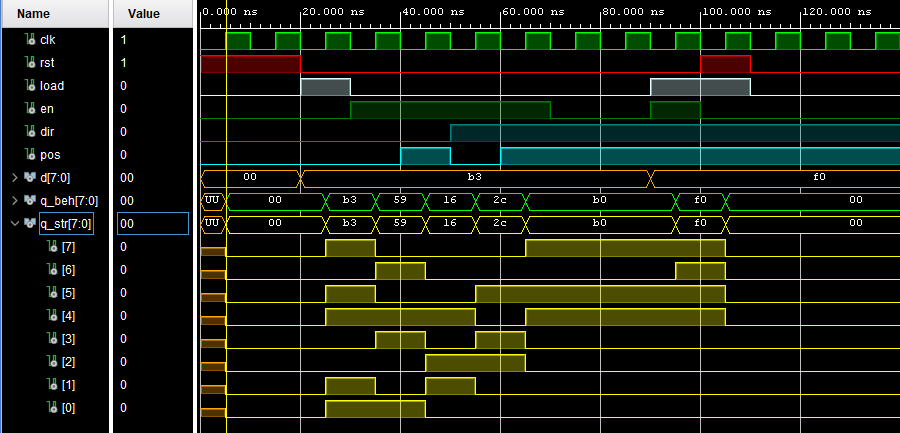
\includegraphics[width=0.95\linewidth]{figure/esercizio4-1/simulazione}
  \caption{Simulazione dello shift register}
  \label{fig:esercizio4-1:simulazione}
\end{figure}

Dopo il reset, con \texttt{load} a \texttt{'1'} e \texttt{d} pari a 0xB3 ($1011\,0011_2$), le due uscite \texttt{q\_beh} e \texttt{q\_str} assumono il valore b3 al fronte di clock successivo. Con \texttt{en} attivo e \texttt{dir} e \texttt{pos} a \texttt{'0'}, il valore diventa 0x59 ($0101\,1001_2$), ossia lo scorrimento a destra di una posizione; con \texttt{pos} a \texttt{'1'} diventa 0x16 ($0001\,0110_2$), a destra di due; con \texttt{dir} a \texttt{'1'} e \texttt{pos} a \texttt{'0'} diventa 0x2C ($0010\,1100_2$), a sinistra di una; infine con \texttt{pos} a \texttt{'1'} diventa 0xB0 ($1011\,0000_2$), a sinistra di due. Il valore 0xB0 resta invariato mentre \texttt{en} è a \texttt{'0'}. Al caricamento simultaneo con \texttt{en} le uscite passano a 0xF0, e all'ultimo impulso di \texttt{rst}, applicato insieme a \texttt{load}, tornano a 0x00. In tutti i passi le due uscite coincidono.

\begin{risultato}
Le uscite \texttt{q\_beh} e \texttt{q\_str} coincidono lungo tutta la simulazione: b3, 59, 16, 2c, b0, f0 e infine 00.
\end{risultato}
